\documentclass[handout]{beamer}
% L'option handout permet de supprimer la barre de navigation

\usepackage[T1]{fontenc}
\usepackage[utf8]{inputenc}
\usepackage[french]{babel}
% Pour utiliser le signe €
\usepackage{eurosym}
% Pour pouvoir insérer des images
\usepackage{graphicx}
\usepackage{wrapfig}
% Gestion des couleurs
\usepackage{color}
\definecolor{QTPurple}{RGB}{61, 68, 160}
% Coloration syntaxique
\usepackage{listings}
\lstset{ 
	language=PHP,
	numbers=left,
	showstringspaces=false, 
	tabsize=4,
	breaklines=true,
	extendedchars=true,
	literate={é}{{\'e}}1 {à}{{\`a}}1 {è}{{\`e}}1 {ç}{{\c c}}1
}

% Un joli thème flat
\usetheme{Rochester}

% Personnalisation du thème
\usecolortheme[named=QTPurple]{structure}
\setbeamertemplate{blocks}[shadow=false]

% Générer une page de titre à chaque début de section
% \AtBeginSection[]
% {
% 	\begin{frame}[plain]
% 	\frametitle{Sommaire}
% 	\tableofcontents[currentsection, hideothersubsections]
% 	\end{frame} 
% }

% Affichage du logo en bas de chaque slide
\logo{
\includegraphics[height=8mm]{images/logo.png}}

% ------------------------------------ %
% -- METADONNÉES DU DOCUMENT --------- %
\title[Quantic]{
	Projet d'électronique\\
	Un réveil intelligent
}
\author{
	Antoine Augusti, Étienne Batise, Jean-Claude Bernard, Thibaud Dauce
}
\date{Janvier 2014}

\titlegraphic{
\includegraphics[height=.2\textheight]{images/logo.png}}

% Début du document
\begin{document}
	
	% Génération de la page de titre
	\begin{frame}[plain]
		\titlepage
	\end{frame}

	% Génération du sommaire
	\begin{frame}[plain]
		\frametitle{Sommaire}
		\tableofcontents
	\end{frame}


	% ////////////////////////////////////////////////// %
	% /// Présentation du projet /////////////////////// %
	\section{Présentation du projet}

	\begin{frame}
	\frametitle{But de notre projet}
	\begin{tabular}{l l}
		\begin{minipage}{0.2\textwidth}
			\begin{center}
				
\includegraphics[width=0.9\textwidth]{images/but.png}
			\end{center}
		\end{minipage}

		\begin{minipage}{0.8\textwidth}
			\begin{itemize}
				\item Interface de programmation du réveil
				\item Au matin, allumage progressif de la lumière et lecture d'un son
				\item Arrêt du réveil lors de l'allumage de la lumière de la pièce
				\item Informations utiles lors du réveil (news, prochains métros, météo)
			\end{itemize}
		\end{minipage}
		
	\end{tabular}
	\end{frame}
	% ///////////////////////////////////////////////////////// %


	% ///////////////////////////////////////////////// %
	% /// Technologies utilisées ///////////////////// %
	\section{Technologies utilisées}

	\subsection{Liste des technologies utilisées}
		\begin{frame}
		\frametitle{Liste des technologies utilisées}

		\begin{tabular}{l l}
			\begin{minipage}{0.2\textwidth}
				\begin{center}
					
\includegraphics[width=0.9\textwidth]{images/outils.png}
				\end{center}
			\end{minipage}

			\begin{minipage}{0.8\textwidth}
				\begin{itemize}
					\item Quelques notions de réseau
					\item De l'électronique !
					\item Des langages de programmation
					\begin{itemize}
						\item technos web : HTML5, CSS3, JavaScript, PHP
						\item Langage Arduino
						\item Raspberry Pi : scripts Bash
					\end{itemize}
				\end{itemize}
			\end{minipage}
			
		\end{tabular}
		\end{frame}

	\subsection{Électronique}
		\begin{frame}
		\frametitle{Électronique}

		\begin{tabular}{l l}
			\begin{minipage}{0.2\textwidth}
				\begin{center}
					
\includegraphics[width=0.9\textwidth]{images/electricite.png}
				\end{center}
			\end{minipage}

			\begin{minipage}{0.8\textwidth}
				\begin{itemize}
					\item Outil de conception : KiCad
					\item Le shield LDR
					\item Alimentation autonome : 7805
					\item La LED rouge
				\end{itemize}
			\end{minipage}
			
		\end{tabular}
		\end{frame}

	\subsection{Raspberry Pi}
		\begin{frame}
		\frametitle{Raspberry Pi}

		\begin{tabular}{l l}
			\begin{minipage}{0.2\textwidth}
				\begin{center}
					
\includegraphics[width=0.9\textwidth]{images/logoRaspberry.png}
				\end{center}
			\end{minipage}

			\begin{minipage}{0.8\textwidth}
				\begin{itemize}
					\item Interface web de gestion du réveil
					\item Affichage des informations au réveil
					\item Scripts réseau
					\item Communication avec la carte Arduino
					\begin{itemize}
						\item Déclenchement du réveil 
						\item Arrêt du réveil 
					\end{itemize}
				\end{itemize}
			\end{minipage}
			
		\end{tabular}
		\end{frame}

	\subsection{Arduino}
		\begin{frame}
		\frametitle{Arduino}

		\begin{tabular}{l l}
			\begin{minipage}{0.2\textwidth}
				\begin{center}
					
\includegraphics[width=0.9\textwidth]{images/logoArduino.png}
				\end{center}
			\end{minipage}

			\begin{minipage}{0.8\textwidth}
				\begin{itemize}
					\item Blah
					\item Blah
					\item Blah
					\item Blah
				\end{itemize}
			\end{minipage}
			
		\end{tabular}
		\end{frame}


	% //////////////////////////////////////////////////// %
	% /// Démonstration ////////////////////////////// %
	\section{Démonstration}

	\begin{frame}
	\frametitle{Démonstration}
		\begin{tabular}{l l}
			\begin{minipage}{0.7\textwidth}
				\begin{center}
					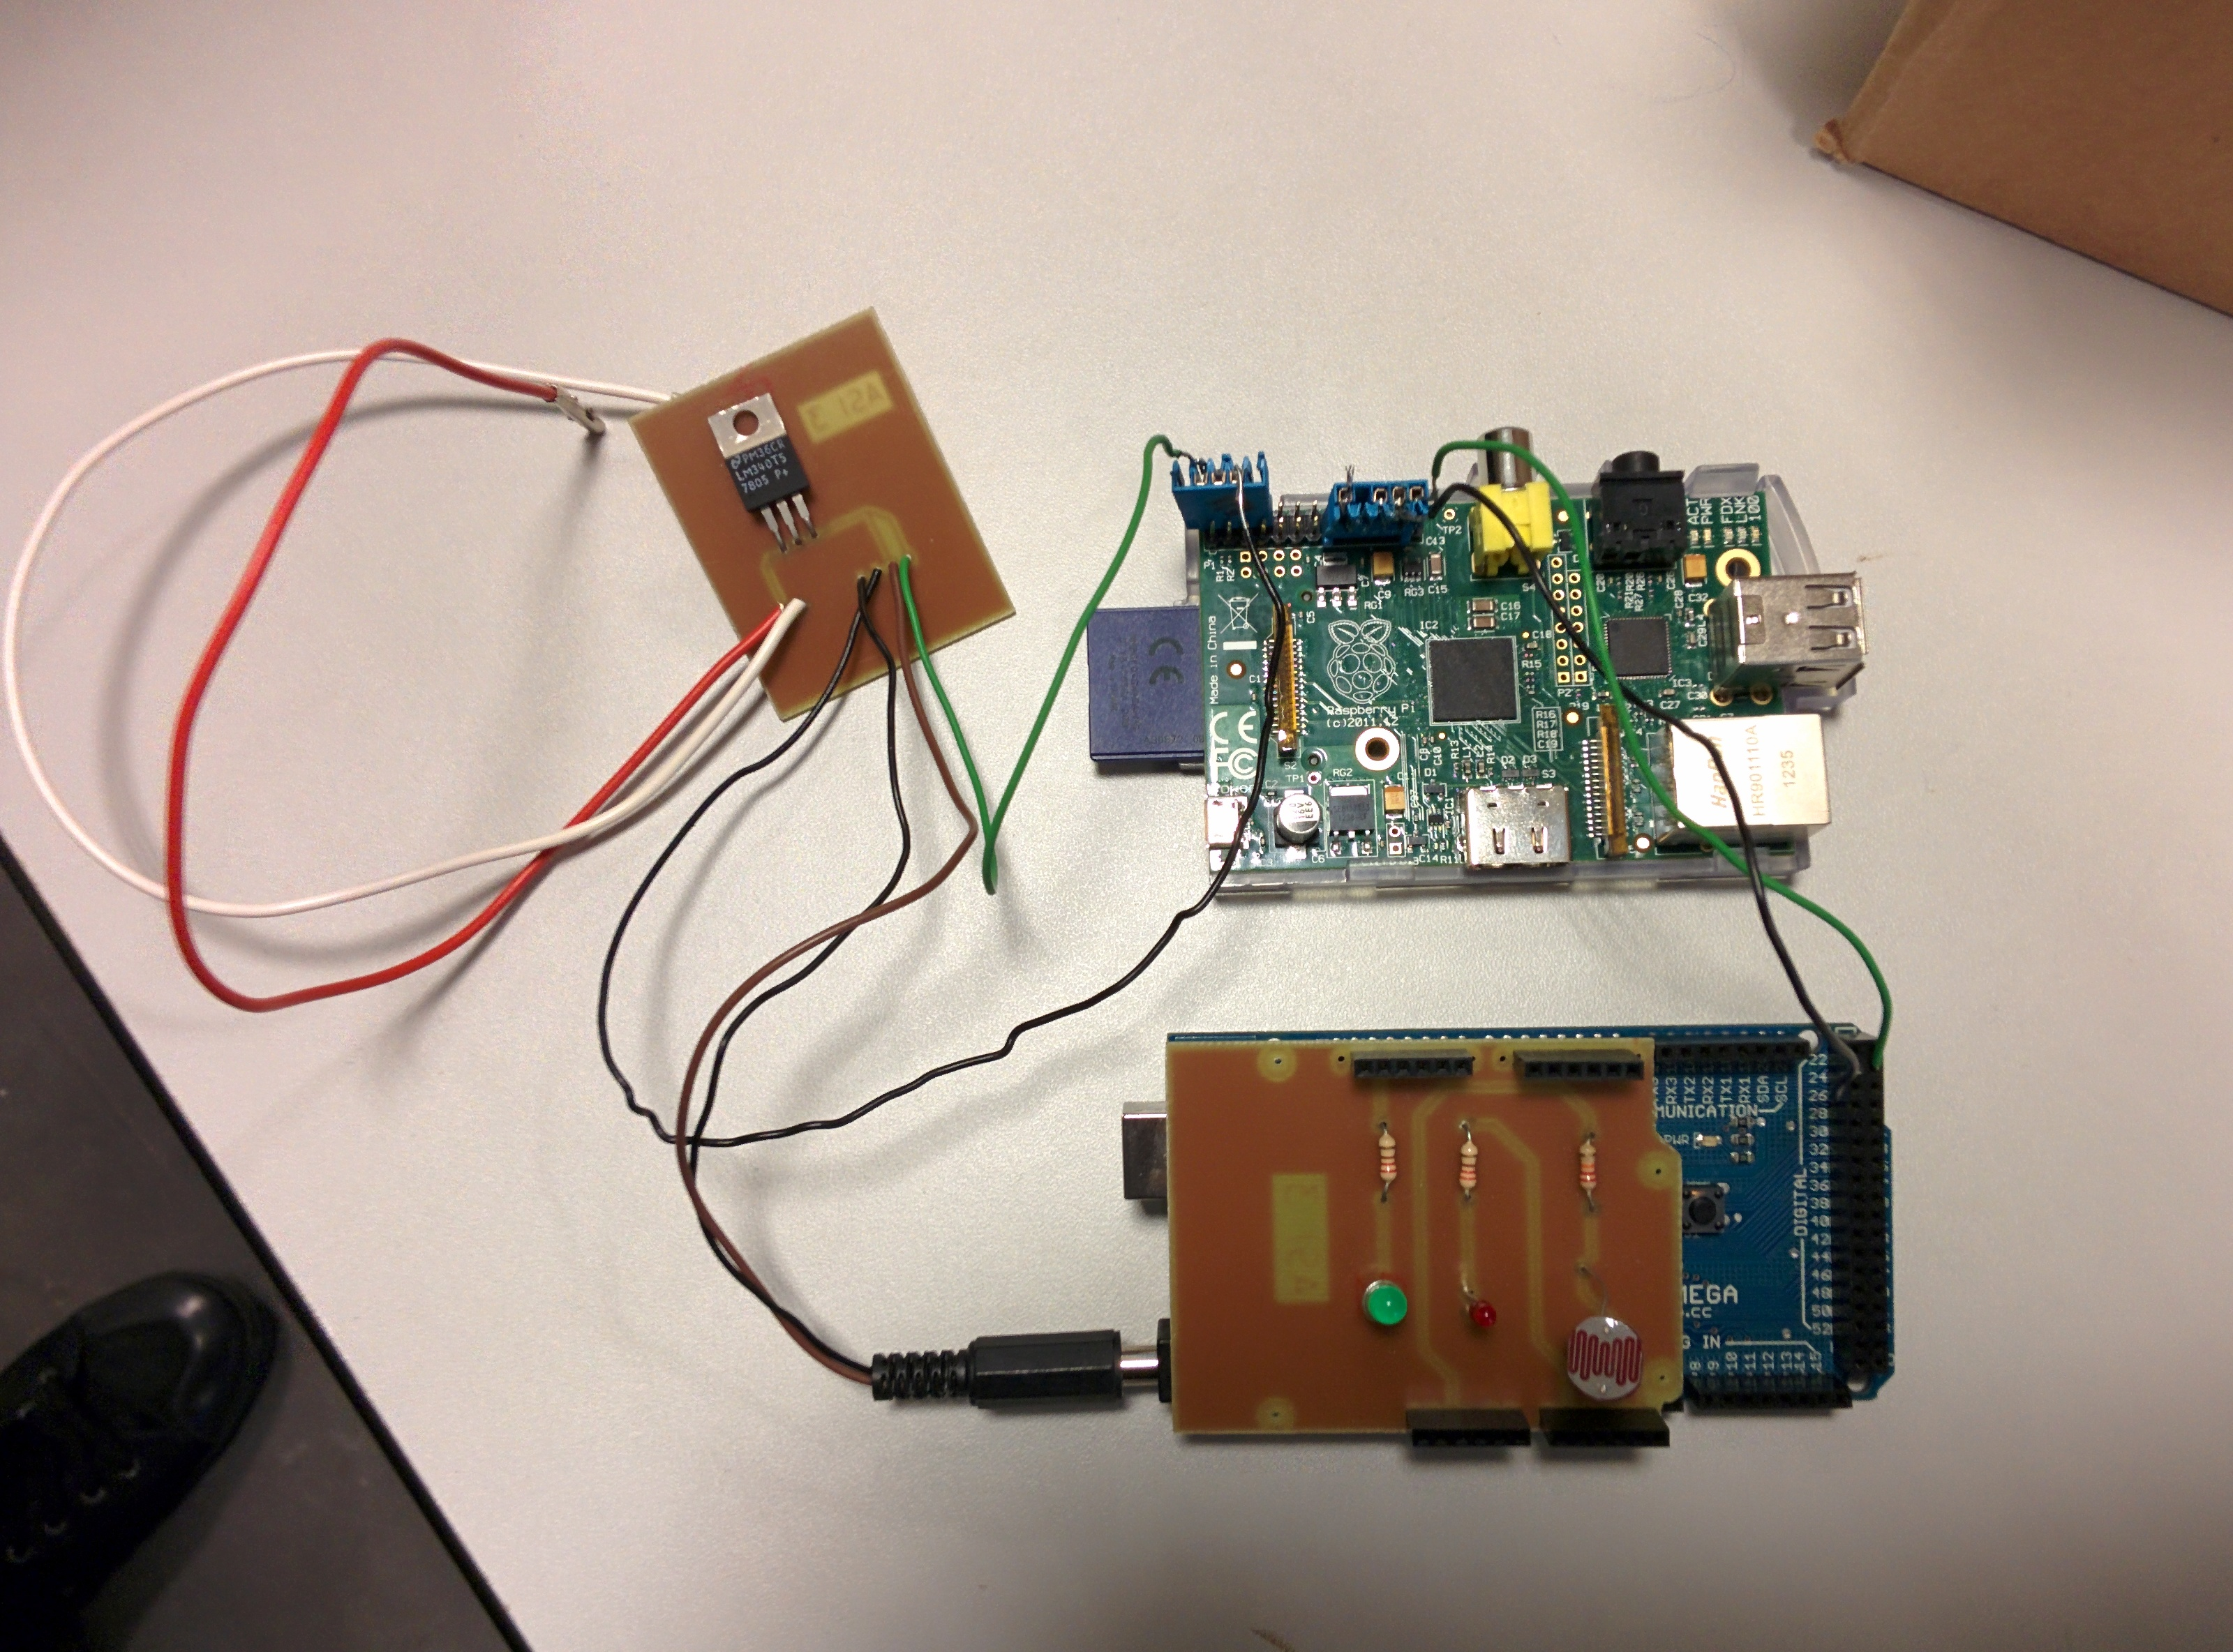
\includegraphics[width=0.7\textwidth]{images/projetFinal.jpg}
				\end{center}
			\end{minipage}

			\begin{minipage}{0.3\textwidth}
				\Huge{Show Time}
			\end{minipage}
			
		\end{tabular}
	\end{frame}

	% ///////////////////////////////////////////// %
	% /// Conclusion ////////////////////////////// %
	\section{Conclusion}

	\begin{frame}
	\frametitle{Conclusion}
		\begin{itemize}
			\item Projet non utilisable en conditions réelles !
			\item Nous avons beaucoup appris :-)
			\item Beaucoup d'améliorations sont encore possibles
		\end{itemize}
	\end{frame}

% Fin du document
\end{document}